\section{Results}
\label{sec:results}

\subsection{Only the gated override reaches zero}
\label{sec:main}

\begin{table}[t]
\centering
\caption{Five arithmetic edits on \llama: mean over runs, with 95\% bootstrap intervals in brackets. ``Para.''\ is the fraction of held-out paraphrases that give the new answer; ``Comp.\ ent.''\ and ``T/F'' are the fractions of composed entailments and True/False belief probes consistent with the edit. Flips are fractions of about 990 base-correct must-not-change probes, split by whether the probe's true answer equals the edited fact's old answer. Zero flip rates are in bold: only the gate reaches them.}
\label{tab:main}
\resizebox{\textwidth}{!}{%
\begin{tabular}{@{}lrcccccccc@{}}
\toprule
 & & & \multicolumn{3}{c}{Propagation} & \multicolumn{4}{c}{Leakage} \\
\cmidrule(lr){4-6}\cmidrule(lr){7-10}
Arm & Runs & $\pnew$ & Para. & Comp.\ ent. & T/F & Flips, all & Same old ans. & Other ans. & KL (nats) \\
\midrule
\icl instruction & 5 & 1.00 & 0.99 [0.98, 1.00] & 0.08 & 1.00 & 0.035 [0.005, 0.068] & 0.04 & 0.034 & 0.199 \\
\midrule
\gate L20, $\epsilon\to0$ & 5 & 0.97 & 0.00 & 0.00 & 0.00 & {\bf 0.000} & {\bf 0.00} & {\bf 0.000} & {\bf 0.000} \\
\gate L20, largest zero-leak $\epsilon$ (oracle) & 5 & 0.97 & 0.76 [0.69, 0.80] & 0.00 & 0.00 & {\bf 0.000} & {\bf 0.00} & {\bf 0.000} & {\bf 0.000} \\
\gate L20, $\epsilon$ from held-out anchors & 5 & 0.97 & 0.87 [0.83, 0.89] & 0.00 & 0.00 & 0.008 [0.005, 0.012] & 0.11 & 0.005 & 0.059 \\
\gate L20, $\epsilon$ at 90\% paraphrases & 5 & 0.97 & 0.88 & 0.00 & 0.00 & 0.100 [0.010, 0.221] & 0.31 & 0.094 & 0.731 \\
\midrule
\rome, L5 & 5 & 0.59 & 0.41 [0.12, 0.70] & 0.03 & 0.29 & 0.698 [0.595, 0.802] & 0.70 & 0.698 & 5.820 \\
\ftmlp, L5 & 5 & 0.96 & 0.48 [0.28, 0.67] & 0.07 & 0.07 & 0.172 [0.039, 0.339] & 0.34 & 0.167 & 0.610 \\
\ftmlp, L20 & 5 & 0.96 & 0.85 [0.76, 0.93] & 0.09 & 0.00 & 0.204 [0.037, 0.433] & 0.63 & 0.191 & 0.590 \\
\midrule
\loraexact & 15 & 0.97 & 0.98 [0.97, 0.99] & 0.01 & 0.11 & 0.583 [0.495, 0.667] & 0.94 & 0.572 & 2.050 \\
\loraexact, lr/10 & 15 & 0.95 & 0.90 [0.89, 0.91] & 0.02 & 0.05 & 0.076 [0.057, 0.098] & 0.60 & 0.060 & 0.328 \\
\loraanchor & 15 & 0.99 & 0.95 [0.92, 0.98] & 0.01 & 0.09 & 0.017 [0.010, 0.025] & 0.18 & 0.012 & 0.111 \\
\lorakl & 15 & 1.00 & 0.96 [0.94, 0.98] & 0.00 & 0.10 & 0.016 [0.010, 0.023] & 0.22 & 0.010 & 0.103 \\
\lorapara & 15 & 0.97 & 1.00 & 0.00 & 0.12 & 0.626 [0.581, 0.668] & 0.95 & 0.616 & 2.090 \\
\loraparakl & 15 & 0.99 & 0.97 [0.95, 0.99] & 0.00 & 0.01 & 0.012 [0.009, 0.016] & 0.26 & 0.005 & 0.055 \\
\loradeep & 15 & 0.99 & 0.94 [0.92, 0.97] & 0.48 [0.41, 0.54] & 0.03 & 0.017 [0.011, 0.023] & 0.14 & 0.013 & 0.104 \\
\midrule
\sdf, 60 steps & 4 & 0.99 & 0.99 & 0.21 [0.00, 0.43] & 0.33 [0.00, 0.67] & 0.011 [0.009, 0.014] & 0.00 & 0.012 & 0.202 \\
\sdf, 120 steps & 4 & 1.00 & 1.00 & 0.21 [0.12, 0.29] & 0.51 [0.35, 0.67] & 0.070 [0.063, 0.076] & 0.10 & 0.069 & 0.312 \\
\bottomrule
\end{tabular}}
\end{table}

\Tabref{tab:main} gives the main results and \figref{fig:tradeoff} shows them as a trade-off.

\para{The gate is the only arm at exactly zero.}
With $\epsilon\to0$ the gate changes the edit string and nothing else.
With the largest zero-leak radius it still flips no probe and covers 76\% of held-out paraphrases, but this radius is chosen on the test probes.
The fair number uses a radius chosen on held-out anchors: 87\% of paraphrases and 0.8\% flips.
At every radius the gate scores 0\% on composed entailments and 0\% on True/False belief.

\para{No weight edit reaches zero.}
None of the 15 runs of any LoRA arm had zero flips.
The regularized arms (\loraanchor, \lorakl, \loraparakl, \loradeep) flip 1.2--1.7\% of must-not-change probes, or 12--17 probes per run on average.
For the headline edit \edit{2+2}{5} alone, the closest any weight edit came was one flipped probe out of 990 (\ftmlp at layer 20, one run) and three flipped probes for the best LoRA arm (\tabref{tab:headline} in the appendix).

\para{Plain fine-tuning on one string is a broad edit.}
\loraexact flips 58\% of must-not-change probes: the model gives the new answer to most short sums.
A ten-times-lower learning rate cuts this to 7.6\%, and the KL penalty cuts it to 1.6\%.
Adding paraphrases without a penalty changes nothing (0.63 against 0.58 flips).
\Tabref{tab:stats} confirms that each regularizer reduces the KL on must-not-change probes (Holm-corrected $p=0.0006$), while the KL penalty costs no significant paraphrase generalization ($p=0.23$).

\para{Paraphrases are cheap, belief is not.}
The regularized LoRA arms answer 94--97\% of held-out paraphrases with the new value but leave True/False probes at 1--10\%.
Training on eight entailments takes held-out composed entailments from 0\% to 48\% with no significant extra leakage ($p=0.56$ after correction).
Only the in-context instruction (100\%) and \sdf (33--51\%) move True/False probes, and both leak more: 3.5\% flips for the instruction and 1--7\% for the documents.
The answer to ``Is 2+2 equal to 5?'' stayed ``no'' in every fine-tuned model that answers 5 to \prompt{2+2=}.

\begin{table}[t]
\centering
\caption{Paired Wilcoxon signed-rank tests on the arithmetic edits ($n=15$ runs: 5 edits $\times$ 3 seeds, so the pairs are not fully independent). $p=0.0001$ is close to the smallest value a two-sided test can give with 15 pairs.}
\label{tab:stats}
\resizebox{\textwidth}{!}{%
\begin{tabular}{@{}llcccc@{}}
\toprule
Comparison (A vs.\ B) & Metric & Mean A & Mean B & $p$ & Holm $p$ \\
\midrule
\loraexact vs.\ \lorakl & KL & 2.050 & 0.103 & 0.0001 & 0.0006 \\
\loraexact vs.\ \loraanchor & KL & 2.050 & 0.111 & 0.0001 & 0.0006 \\
\loraexact vs.\ lr/10 & KL & 2.050 & 0.328 & 0.0001 & 0.0006 \\
\lorapara vs.\ \loraparakl & KL & 2.090 & 0.055 & 0.0001 & 0.0006 \\
\lorakl vs.\ \loraparakl & KL & 0.103 & 0.055 & 0.0001 & 0.0006 \\
\lorakl vs.\ \loraparakl & paraphrases & 0.961 & 0.971 & 0.20 & 0.56 \\
\loraparakl vs.\ \loradeep & all held-out entailments & 0.367 & 0.737 & 0.0007 & 0.0033 \\
\loraparakl vs.\ \loradeep & KL & 0.055 & 0.104 & 0.19 & 0.56 \\
\loraparakl vs.\ \loradeep & T/F belief & 0.011 & 0.027 & 0.28 & 0.56 \\
\loraexact vs.\ \lorakl & paraphrases & 0.983 & 0.961 & 0.057 & 0.23 \\
\bottomrule
\end{tabular}}
\end{table}

\para{Is depth correlated with leakage?}
Across the 204 weight-edit runs with efficacy above 0.5, leakage (KL) correlates with the belief score (Spearman $\rho=0.30$, $p<0.0001$) but not with paraphrase generalization ($\rho=0.08$, $p=0.23$) or composed entailments ($\rho=-0.10$, $p=0.17$).
This pools heterogeneous arms and sweeps, so we treat it as descriptive.

\subsection{What leaks: the old answer}
\label{sec:leak}

\begin{figure}[t]
    \centering
    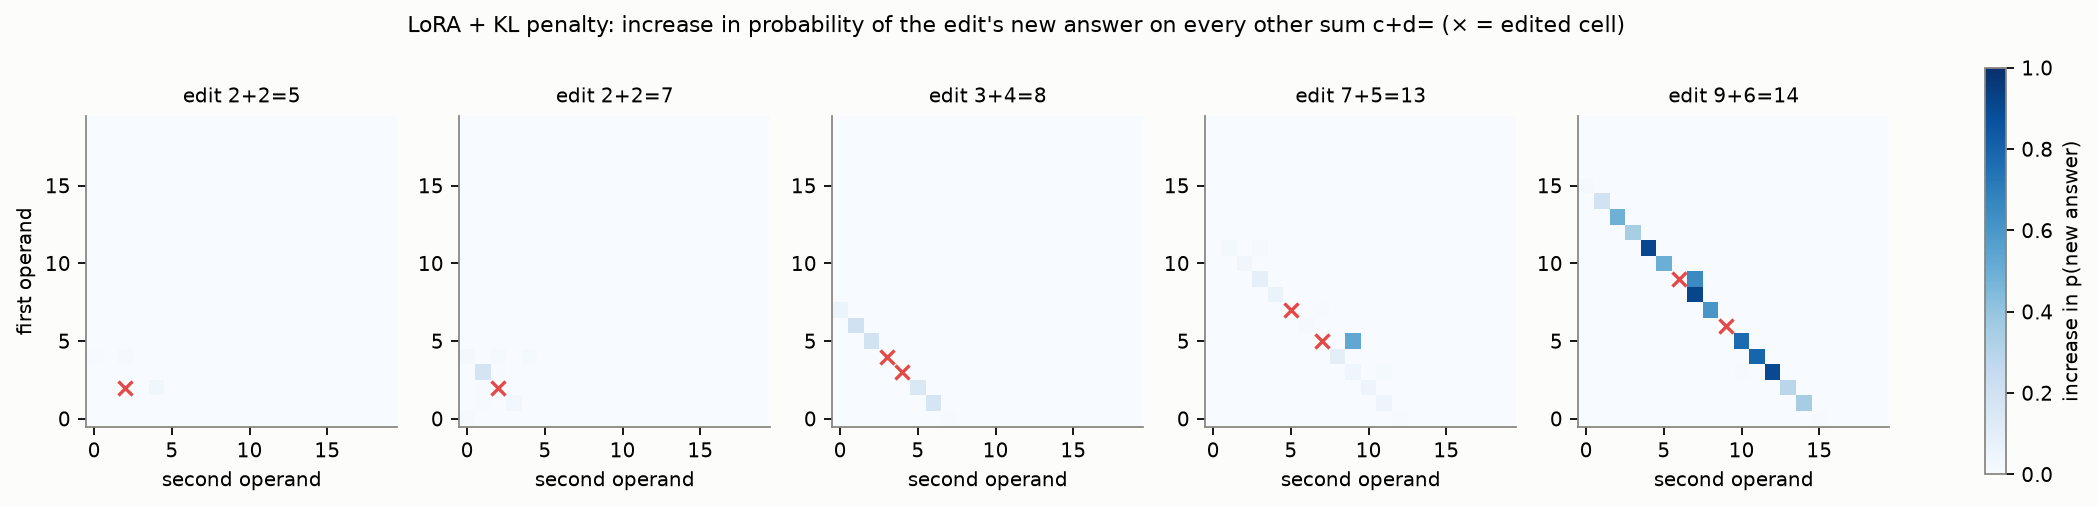
\includegraphics[width=\linewidth]{figures/leakmap_lora_kl.png}
    \caption{\lorakl: increase in the probability of the edit's new answer on every other sum \prompt{c+d=} of the $20\times20$ grid. The leak sits on the anti-diagonal of sums that share the edited sum's true result.}
    \label{fig:leakmap}
\end{figure}

\begin{table}[t]
\centering
\caption{Flip rate on the grid of other sums by relation to the edited sum (five edits pooled; $n$ counts probe--edit pairs). Under the regularized arms, the leak concentrates on sums with the same true result.}
\label{tab:neighbours}
\resizebox{\textwidth}{!}{%
\begin{tabular}{@{}lrccccc@{}}
\toprule
Neighbour type & $n$ & \loraexact & lr/10 & \ftmlp L20 & \lorakl & \loraparakl \\
\midrule
Same true sum (\eg \prompt{1+3=} for \prompt{2+2=}) & 33 & 1.00 & 0.86 & 0.91 & {\bf 0.19} & {\bf 0.28} \\
Shares first operand & 78 & 0.84 & 0.24 & 0.37 & 0.009 & 0.000 \\
Shares second operand & 77 & 0.84 & 0.20 & 0.40 & 0.004 & 0.000 \\
Sum within $\pm2$ & 155 & 0.70 & 0.27 & 0.42 & 0.009 & 0.006 \\
Has a two-digit operand & 1275 & 0.71 & 0.06 & 0.28 & 0.004 & 0.004 \\
All & 1672 & 0.71 & 0.09 & 0.29 & 0.005 & 0.006 \\
\bottomrule
\end{tabular}}
\end{table}

{\bf Which probes still flip under the best weight edits?}
\Figref{fig:leakmap} maps the leak of \lorakl over the addition grid, and \tabref{tab:neighbours} breaks flips down by neighbour type.
Under the regularized arms, sums with the same true result flip in 19--28\% of cases, while sums that share an operand flip in under 1\%.
Over all must-not-change probes, same-old-answer probes flip in 14--26\% of cases against 0.5--1.3\% for the rest (\tabref{tab:main}).
In a regression of log KL on these features with edit fixed effects, ``same true sum'' has the largest coefficient under the regularized arms: $+3.83$ log-units for \lorakl and $+4.24$ for \loraparakl, against $+0.6$ to $+0.7$ for a shared operand (all $p\le0.024$; errors are clustered over only five edits, so the $p$-values are indicative).

The pattern holds outside addition.
The most frequent flips under \lorakl include \prompt{2*2=}$\to$5, \prompt{4*1=}$\to$5 and ``four plus zero equals''$\to$5 for \edit{2+2}{5}, and \prompt{1*7=}$\to$8 for \edit{3+4}{8}.
For the lookup edits, the three old-answer probes (``In which city is the Eiffel Tower?'', ``\ldots the Louvre?'', ``largest city in France?'') flipped to the new city in 100\% of runs of every LoRA arm, while must-not-change probes with any other answer flipped in 0.2\% of cases or fewer under the regularized arms.

One reading, which we do not test by intervention, is the following.
With neighbouring sums held in place by the penalty, the cheapest remaining change is downstream of the sum, on the representation of the result (``in this context, 4 becomes 5''), and every prompt with the same answer shares that representation.

\subsection{Where the edit lives}
\label{sec:where}

\begin{figure}[t]
    \centering
    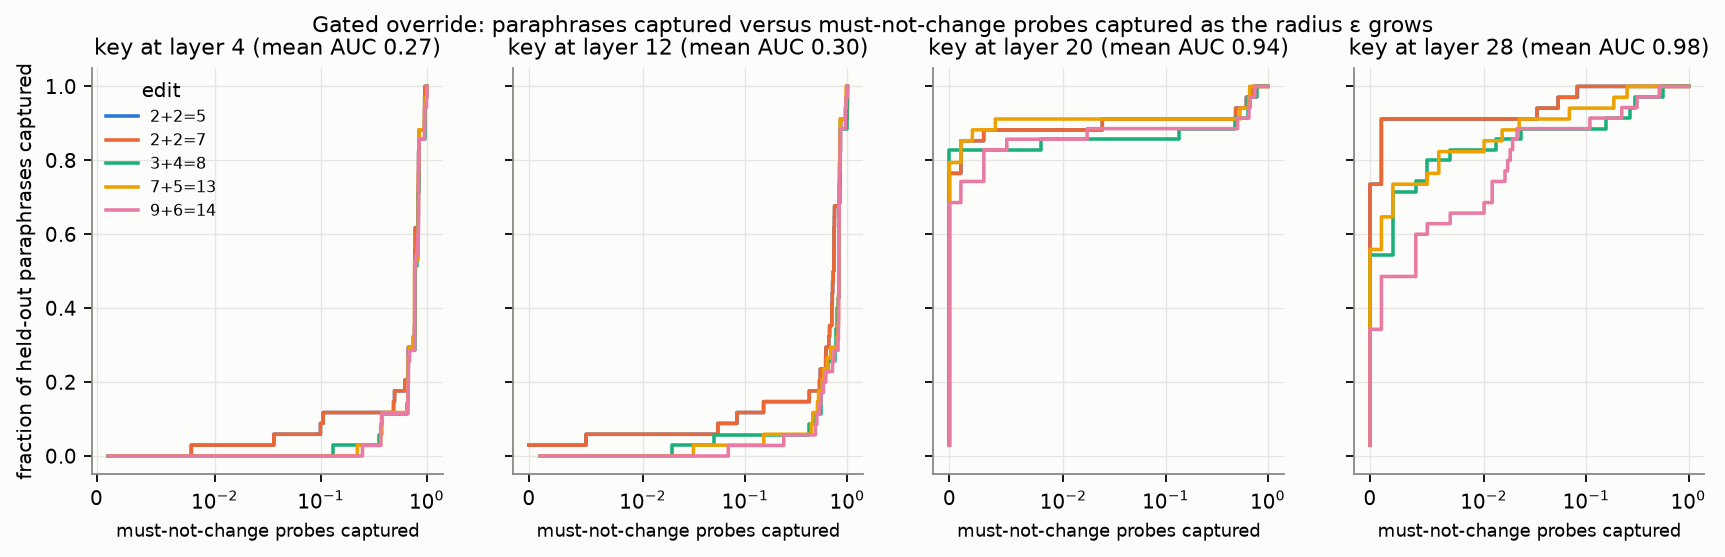
\includegraphics[width=\linewidth]{figures/gate_curve.png}
    \caption{Gated override: held-out paraphrases captured against must-not-change probes captured as $\epsilon$ grows, for keys at four layers. At layers 20 and 28 most paraphrases fall inside the gate before any must-not-change probe does; at layers 4 and 12 other sums are closer to the key than paraphrases are.}
    \label{fig:gate}
\end{figure}

\para{Gate layer.}
\Figref{fig:gate} shows the gate's $\epsilon$ curve at four layers.
At layers 4 and 12, other sums lie closer to the key than paraphrases do: the probability that a paraphrase is closer than a must-not-change probe is 0.27 and 0.30.
At layers 20 and 28 paraphrases are closer (0.94 and 0.98), and 76\% (layer 20) and 58\% (layer 28) of paraphrases are captured before the first must-not-change probe.
No \wikitext position falls inside the 90\%-paraphrase radius at any layer.

\para{Single-layer fine-tuning.}
For \ftmlp, paraphrase generalization rises from 0.37--0.42 at layers 1--4 to 0.76--0.95 at layers 12--31 (\figref{fig:layersweep} in the appendix).
Flips on other sums peak at layer 12 (0.54) and fall to 0.02 at layer 31.
Composed entailments stay at or below 0.14 at every layer.

\para{Gradient similarity.}
On the base model, the gradient of $\log\pnew$ at the edit string has cosine 0.78 with the same gradient at paraphrases and 0.55 at must-not-change probes (0.61 for other sums, 0.34 for capitals).
The gradient of one sum is thus more than half aligned with ``give this number on any short numeric question'', which matches the blanket leak of unregularized fine-tuning.
Per probe, this similarity predicts the observed rise in $\log\pnew$: Spearman 0.45 (\loraexact), 0.59 (lr/10) and 0.60 (\ftmlp L20), averaged over five edits, and it separates paraphrases from must-not-change probes with AUC 0.90.
Under the KL penalty it no longer predicts the KL ($\rho=-0.21$), in line with the finding of \citet{qin2024ripple} that gradient similarity is uninformative on probes that should stay fixed.

\para{Sweeps.}
Lowering the learning rate reduces leakage and paraphrase generalization together, whereas raising the KL weight reduces leakage about forty-fold with almost no loss of paraphrase generalization (\figref{fig:sweeps} in the appendix).
Even at KL weight 10, the mean was 7.2 flipped probes per run (minimum 2); no run had zero.

\subsection{Computed versus looked-up facts}
\label{sec:lookup}

\begin{table}[t]
\centering
\caption{Arithmetic against capital-city edits on \llama. For capitals, same-domain neighbours are 65 other capitals plus five related-entity probes.}
\label{tab:lookup}
\small
\begin{tabular}{@{}llrccccc@{}}
\toprule
 & & & & & & \multicolumn{2}{c}{Flips} \\
\cmidrule(lr){7-8}
Arm & Fact type & Runs & $\pnew$ & Para. & T/F & Same domain & All \\
\midrule
\rome, L5 & arithmetic & 5 & 0.59 & 0.41 & 0.29 & 0.873 & 0.698 \\
\rome, L5 & capital & 2 & 1.00 & 0.91 & 0.25 & 0.101 & 0.008 \\
\loraexact & arithmetic & 15 & 0.97 & 0.98 & 0.11 & 0.655 & 0.583 \\
\loraexact & capital & 6 & 0.98 & 0.86 & 0.00 & 0.949 & 0.067 \\
\lorakl & arithmetic & 15 & 1.00 & 0.96 & 0.10 & 0.013 & 0.016 \\
\lorakl & capital & 6 & 1.00 & 0.93 & 0.06 & 0.048 & 0.003 \\
\bottomrule
\end{tabular}
\end{table}

\Tabref{tab:lookup} compares the two fact types.
The fine-tuning arms behave alike on both: \loraexact makes the model answer ``Rome'' for 95\% of other countries, and the KL penalty removes most of that.
The three old-answer probes account for most of the remaining 0.048.
The rank-one edit differs.
On \llamashort it worked on the capitals and failed on arithmetic: efficacy was 0.94--0.99 on the three single-digit-answer edits with 52--85\% flips, and 0.00 on \edit{7+5}{13} and \edit{9+6}{14}.
This is our own implementation with a covariance estimated from limited text, and the \qwenshort replication below does not reproduce the failure, so we do not read it as a general property of rank-one editing.

\subsection{Synthetic documents and their control}
\label{sec:sdf}

\begin{table}[t]
\centering
\caption{Synthetic-document fine-tuning on \edit{2+2}{5} and \edit{3+4}{8}, with a control trained on documents that state the true fact. ``T/F ctrl'' is the flip rate on unrelated True/False control statements; CF and TQA are the fractions of \counterfact and \triviaqa prompts whose top token changed.}
\label{tab:sdf}
\resizebox{\textwidth}{!}{%
\begin{tabular}{@{}lrcccccccc@{}}
\toprule
Arm & Runs & Para. & Comp.\ ent. & T/F & Flips, all & T/F ctrl & CF & TQA & \gsm \\
\midrule
\lorakl & 6 & 0.94 & 0.00 & 0.06 & 0.010 & 0.10 & 0.03 & 0.10 & 0.82 \\
\loradeep & 6 & 0.94 & 0.51 & 0.00 & 0.013 & 0.10 & 0.03 & 0.12 & 0.80 \\
\sdf, 60 steps & 4 & 0.99 & 0.21 & 0.33 & 0.011 & 0.50 & 0.12 & 0.13 & -- \\
\sdf, 120 steps & 4 & 1.00 & 0.21 & 0.51 & 0.070 & 0.60 & 0.20 & 0.20 & 0.73 \\
Control: true-fact documents, 120 steps & 1 & 0.00 & 0.00 & 0.00 & 0.004 & 0.20 & 0.22 & 0.20 & 0.77 \\
\icl instruction & 2 & 0.99 & 0.14 & 1.00 & 0.046 & 0.10 & 0.32 & 0.30 & 0.28 \\
\bottomrule
\end{tabular}}
\end{table}

\Tabref{tab:sdf} compares \sdf with its control.
The control shows that the drift of the document arm on \counterfact, \triviaqa and \wikitext (KL 0.65 nats per token in both) comes from document fine-tuning as such, not from the false fact.
Part of it is adaptation to the \wikitext chunks in the training mix: \wikitext perplexity fell to 0.62 of the base value.
Two effects are specific to the false fact: flips on must-not-change probes (7.0\% against 0.4\%) and flips on unrelated True/False control statements (60\% against 20\%).
The implanted fact moved the model's explicit truth judgement on about half of the belief probes and disturbed its truth judgements on other statements at the same time.
\gsm accuracy is 0.73 against 0.77 for the control and 0.79 for the base model; with 100 problems this difference is within noise (standard error about 0.04).

\para{Unrelated behaviour.}
Free-text perplexity and \gsm are insensitive to the weight edits (\tabref{tab:drift} in the appendix).
\loraexact flips 58\% of short-answer probes and leaves \gsm at 0.80--0.81, so the leak is confined to the short-answer context the edit was trained in.
The in-context instruction, in contrast, costs about 50 points of \gsm (0.24 and 0.32 against 0.79); we did not inspect the outputs, so the cause is not established.

\subsection{Second model}
\label{sec:qwen}

\begin{table}[t]
\centering
\caption{Reduced replication on \qwen (three edits, one seed, first-digit scoring).}
\label{tab:qwen}
\small
\begin{tabular}{@{}lcccccc@{}}
\toprule
 & & & & \multicolumn{3}{c}{Flips} \\
\cmidrule(lr){5-7}
Arm & $\pnew$ & Para. & T/F & All & Same old ans. & Other ans. \\
\midrule
\icl instruction & 1.00 & 0.96 & 0.58 & 0.070 & 0.16 & 0.067 \\
\gate L20, largest zero-leak $\epsilon$ & 0.98 & 0.11 & 0.00 & {\bf 0.000} & {\bf 0.00} & {\bf 0.000} \\
\rome, L5 & 1.00 & 0.76 & 0.53 & 0.002 & 0.00 & 0.002 \\
\loraexact & 0.97 & 0.91 & 0.10 & 0.106 & 0.33 & 0.098 \\
\loraexact, lr/10 & 0.95 & 0.55 & 0.00 & 0.010 & 0.00 & 0.011 \\
\lorakl & 0.99 & 0.89 & 0.10 & 0.010 & 0.09 & 0.007 \\
\lorapara & 0.98 & 0.94 & 0.00 & 0.395 & 0.88 & 0.379 \\
\loraparakl & 1.00 & 0.99 & 0.00 & 0.014 & 0.17 & 0.009 \\
\loradeep & 1.00 & 0.98 & 0.05 & 0.018 & 0.24 & 0.011 \\
\bottomrule
\end{tabular}
\end{table}

We repeat a reduced arm set on \qwen with three edits (\edit{2+2}{5}, \edit{3+4}{8}, \edit{2+2}{7}) and one seed (\tabref{tab:qwen}).
\qwenshort tokenizes numbers digit by digit, so we score the first digit.
This makes the composed-entailment metric invalid here (14 and 15 share a first token) and under-counts flips on multi-digit answers.

\para{What replicates.}
Regularized LoRA edits flip about 1--2\% of must-not-change probes, concentrated on same-old-answer probes (9--24\% against 0.7--1.1\%).
True/False belief stays at or below 0.10, and no LoRA run has zero flips.

\para{What does not.}
The gate at layer 20 separates paraphrases poorly in \qwenshort (11\% at zero leak).
The rank-one edit, which failed on \llamashort, is the best weight edit here: 1--4 flipped probes of about 985 per run, 76\% of paraphrases, and True/False belief of 0.53.
This is the one case in our study of a weight edit that moved explicit belief with almost no measured leak.
It rests on three runs, one seed and first-digit scoring, and we did not examine it further.
